\chapter{Conclusion}
\section{Results}
\label{sec:conc-results}
\subsection{Technology Research}
The first result of this thesis is the documentation of the technology research,
which results in gathered knowledge that is further being required for this
thesis.  It gives an insight in messaging fundamentals and  takes a closer look
to Apache Kafka and related topics.

\subsection{Protocol Implementation}

A fundamental result of this thesis is the implementation of the Apache Kafka
protocol in Haskell. The design decision of separating protocol related code
from the broker implementation leads to an isolated product which now can be used
as library for different projects. The code is provided through an \fnurl{open sourced
repository}{https://github.com/hmb-ba/protocol} for further development.

A complete implementation of the Apache Kafka Protocol would go beyond the scope
of this thesis as the focus lies not only in implementing the protocol but also
to provide broker functionality. Thus, most important is the ability to produce
and fetch messages. In order to provide compatibility to Apache Kafka clients
the Metadata API is required too. This is, because it is the first part of the
process of producing or consuming messages whereas it will request information
about the broker and provided topics. The following list gives an overview of
what part of the protocol is implemented and what remains open:

\begin{itemize}
    \item Metadata API
    \begin{itemize}
        \tick Topic Metadata Request
        \tick Metadata Response
    \end{itemize}
    \item Produce API
    \begin{itemize}
        \tick Produce Request
        \tick Produce Response
    \end{itemize}
    \item Fetch API
    \begin{itemize}
        \tick Fetch Request
        \tick Fetch Response
    \end{itemize}
    \item Offset API
    \begin{itemize}
        \fail Offset Request
        \fail Offset Response
    \end{itemize}
    \item Offset Commit/Fetch API
    \begin{itemize}
        \fail Consumer Metadata Request
        \fail Consumer Metadata Response
        \fail Offset Commit Request
        \fail Offset Commit Response
        \fail Offset Fetch Request
        \fail Offset Fetch Response
    \end{itemize}
\end{itemize}

\subsection{Haskell Message Broker}

The main approach of this work is the implementation of a message broker in
Haskell. The resulting application provides a server with basic functionality in
handling requests via network and persisting messages. The broker is fully Kafka
compatible as it is based on the protocol implementation.  In comparison to
original Apache Kafka there are of course a lot of features missing to offer the
same functionality. Furthermore as the scope of this thesis lies on a single
broker system, there is no support for broker replication yet. Nevertheless the
provided Haskell Message broker is a prototype which shows feasibility of
developing a similar system in a fully-fledged functional program language as
Haskell is. The following list gives an overview what features the broker system
already provides and what remains open in the particular area.

Produce API:
\begin{itemize}
        \tick Publishing messages to specific topic and partition
        \tick Publishing to multiple topics and partitions per request
        \tick Support batched messages
        \fail Configurable Acknowledgements and Timeout
\end{itemize}

Fetch API:
\begin{itemize}
        \tick Consuming messages of a specific topic and partition depending on given offset
        \fail Support consuming from multiple topics and partitions per request
        \fail Support configurable min and max bytes for fetched data
        \fail Support consumer groups
        data is available
\end{itemize}

Metadata API:
\begin{itemize}
        \tick Fetching available topic names from broker
        \tick Include broker information
        \fail Include partition status
        \fail Include replication information
\end{itemize}

Persistence (Log):
\begin{itemize}
        \tick Persist messages in topic-partition specific log structure
        \tick Read messages from log, optimized with index file
        \tick Provide LogManager for handling files and directories structure
        \fail Wirte Index to disk and rebuild the memory after the broker is restarted
        \fail Data retention, whereas old data is discarded after fix period of
            time or Kafka's log compaction is applied. 
\end{itemize}

\newpage
\section{Evaluation}

After highlighting the implemented features above, the question about
performance still remains. Is the provided prototype potentially faster than the
original Apache Kafka or has it near the same throughput? Or are we still fare
away from any approximation to the impressive performance of the reference
system? This chapter describes the environment and tools with which the systems
are tested.  It also gives insight in early stress tests which were very useful
in finding network related bugs. Additional benchmarks are defined to
demonstrate the performance of the final version of the Haskell message broker.
For comparison, the original Apache Kafka system is involved to the benchmarks
by running the equivalent tests on same hardware.

\subsection{Test Setup}

The following tests and benchmarks are performed with one the following hardware
setup:

Broker Server:
\begin{verbatim}
Intel(R) Xeon(R) CPU E3-1245 v3 @ 3.40GHz
One 7200 RPM SATA drive
16GB of RAM
1Gb Ethernet 
\end{verbatim}

Client Hardware:
\begin{verbatim}
Intel(R) Core(TM) i7-2720QM CPU @ 2.20GHz
One SSD SATA drive
16GB of RAM 
1Gb Ethernet
\end{verbatim}

\subsection{HMB Performance Producer}
\label{conc-eval-hmbperformanceprod}

The HMB performance producer is a simple console application used for stress
tests to the broker system. It can be used to generate messages of a given size
and batch them into a single request. It then repeatedly calls the client
library function sendRequest to pack, encode and send the request. The following
code shows the simplified main function:

\begin{lstlisting}
import qualified System.Entropy as E

main = do 
    -- Socket setup 
    -- ....

    -- Get numberOfBytes and batchSize as variable input 
    -- ....

    randBytes <- E.getEntropy numberOfBytes 
    let batch = [randBytes | x <- [1..batchSize]]

    replicateM_ 1000000 (sendRequest sock req) 
    putStrLn "done produce"
    return ()

\end{lstlisting}

\subsection{Kafka Performance Producer}
\label{conc-eval-kafkaperformanceprod}

The \fnurl{Kafka Performance Producer}
{https://github.com/apache/kafka/blob/trunk/clients/src/main/java/org/apache/kafka/clients/tools/ProducerPerformance.java}
is a official product of Apache Kafka to systematically test their broker
system. It is a wrapper around the original Kafka producer client for producing
as much messages as possible. It provides many \fnurl{configuration options}
{http://kafka.apache.org/documentation.html\#newproducerconfigs} for specific
benchmarks. Because the Haskell message broker offers Kafka compatibility, this
performance producer can also be used as an alternative to the HMB performance
producer to test.

The following listing shows the setup for the benchmarks of this thesis, values
in in brackets [ ] are placeholders for the relevant parameters for the
benchmarks.

\begin{verbatim}
Start Zookeeper
>bin/zookeeper-server-start.sh config/zookeeper.properties

Start Kafka Node 
> bin/kafka-server-start.sh config/server.properties

Create Test Topic [TopicName] on broker server with [IP], 
one partition, no replication: 
>bin/kafka-topics.sh --zookeeper [IP]:2181 
    --create --topic [TopicName] --partitions 1 --replication-factor 1

Start single threaded producing benchmark: 
> bin/kafka-run-class.sh org.apache.kafka.clients.tools.ProducerPerformance 
    [TopiName] [NumberOfMessages] [MessageSize] -1 acks=1 
    bootstrap.servers=[IP]:[Port] buffer.memory=67108864 batch.size=[BatchSize]
\end{verbatim}


%\subsection{Test tools}
%\subsubsection{Wireshark}
%Wireshark is used to track tcp streams of ongoing network communication. For the
%To test network throughput and analyze transmitted tcp packaged the tool
%Wireshark is used. 

%\begin{figure}[H]
%    \centering
%    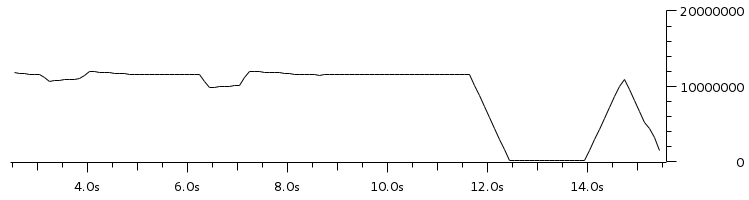
\includegraphics[width=0.85\textwidth]{images/benchmark/bench-1000-1-eth.png}
%    \caption{Example getting tcp throughput graph for specific benchmark test}
%\end{figure}

%\subsubsection{Iptraf-ng}

\newpage
\subsection{Early stress tests}

An early version of the broker provided a console client which produced messages
per console input. This setup demonstrated that encoding/decoding of a request
worked. Also the different broker layers have done their job well.  Later in the
construction phase of the broker, tests which repeatedly send a large amount of
requests in short period of time where introduced. This kind of stress test is
very useful to test network related bugs and performance lacks. The following
table lists some of the major issues, that were exposed: 

\begin{table}[H]
\begin{tabular}{|p{4cm}|p{5cm}|p{6cm}|}
\hline
{\bf Exposed Issue}                                                                                  & {\bf Cause}                                                                                                                                                                                                                 & {\bf Solution}                                                                                                                                                                                                                                                                                    \\ \hline
Dramatically slowdown after short period of time                                                       & TCP Zero Window - Socket receive buffer of broker full                                                                                                                                                                      & Broker application was to slow in receiving, parsing and handling incoming requests. Threading concept need to be optimized (see \ref{sec:impl-broker-threading}). The process of parsing an incoming request need to be swap out to another thread, so that the network receive thread can reduce socket buffer fast enough. \\ \hline
Parsing from socket error "not enough bytes"  when testing over network
interface instead of loopback. & The \lstinline{len} argument to the
\lstinline{recv} system call is merely the upper bound on the received length
(e.g. the size of the target buffer); the call may produce less data than asked
for & Introduced function which checks if really the exact amount of bytes is
read. If not, the \lstinline{recv} call is repeated until all requested bytes are present (see details in \ref{sec:impl-broker-socket-receive}).                                                                                                                                              \\ \hline
Throughput drop when producing larger request with nested list
& Issue in encoding a request, called \lstinline{runPut} on each sub element and
appended to a whole.
& No appending of parsed sub elements. Restructure encode module by running
\lstinline{runPut} at latest point in time. This resulted in factor 2 of performance in building requests (see \ref{sec:impl-prot-encoding}).                                                                                                                                      \\ \hline
Very slow performance in persisting messages to the log (file system).                                 & No state and batching at broker side. Each incoming message ended in multiple file accesses which slowed down the whole process.                                                                                                                                & Messages need to be sum up to larger chunks of bytes. After defined period of time or amount of bytes, multiple messages need to be flushed to disk at once (see details of different approaches in \ref{sec:impl-broker-log}).                                                                                                                                      \\ \hline
\end{tabular}
\end{table}
\captionof{table}{Uncovered issues in early stress tests}


\subsection{Profiling}
When dealing with thousands of request per seconds, function with high complexity
can cause terribly bottlenecks. A method to analyze Haskell code for
potentially slow functions is time and allocation profiling provided by GHC.

TODO
-- Setup?
-- Results 

\subsection{Producer Benchmark "Effect of Message Batch size"}
\label{sec:conc-benchmark-1}

The goal of this benchmark is to analyze the network throughput between producer
client and broker system.  The focus lies on the effect of changing the batch
size at producer client to the resulting transmission of bytes per second. The
batch size determines the amount of bytes for which messages will be packed
together and sent to broker as single request for efficiency.  Increasing the
batch size requires more memory. The size of a single message is fixed to 100
bytes, because it is the more interesting case for a messaging system
(generally). It is easy to get good throughput in MB/sec if the messages are
large, but much harder to get good throughput when the messages are small, as
the overhead of processing each message dominates.

Calculation batch size in bytes:
\begin{verbatim}
    Messages Batched * (Message Size + Message Overhead) + Request Overhead 
\end{verbatim}

\subsubsection{Conditions}
\begin{table}[H]
\begin{tabular}{|l| p{12cm}|} \hline
{\bf Message Size}   & 100 Bytes \\ \hline
{\bf Batch Size [B]} & 195 | 1387 | 8192 | 16384 (Kafka default) | 56769 \\ \hline
{\bf Tested Clients} &
    \begin{itemize}
        \item Kafka PerformanceProducer 2.10-0.8.2.0, single threaded
        \item HMB Producer, single threaded
    \end{itemize}\\ \hline
{\bf Tested Brokers} &
    \begin{itemize}
        \item Kafka Broker 2.10-0.8.2.0, no replication, one partition
        \item HMB Broker, no replication, one partition
    \end{itemize}\\ \hline
{\bf Measurement} & Resulting TCP throughput over a period of 10 seconds, analyzed with
    Wireshark. \\ \hline
{\bf Scenarios} & Producing as much messages as possible from client (left) to broker (right).
    The size of messages batched together varies in defined steps.
    \begin{enumerate}
        \item Kafka Performance Producer $\rightarrow$ Kafka Broker
        \item Kafka Performance Producer $\rightarrow$ HMB Broker
        \item HMB Producer $\rightarrow$ Kafka Broker
        \item HMB Producer $\rightarrow$ HMB Broker
    \end{enumerate} \\ \hline
\end{tabular}
\end{table}
\captionof{table}{Benchmark conditions "Effect of Producer Batch size"}
\newpage
\subsubsection{Results}
The results fora each specific scenarios are given below. The graph shows the
TCP throughput in bytes in period of ten to twenty seconds.

Scenario 1, Kafka $\rightarrow$ Kafka:

\begin{table}[H]
\centering
\begin{tabular}{|l|l|l|} \hline
195 (1 Msg) & 1387 ($\sim$10 Msgs)& 8192 ($\sim$65 Msgs)\\ \hline
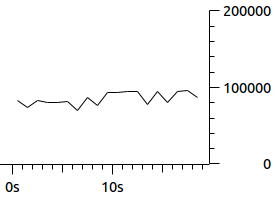
\includegraphics[width=0.25\textwidth]{images/benchmark-1/benchmark-1-s1-bs195.png}
&
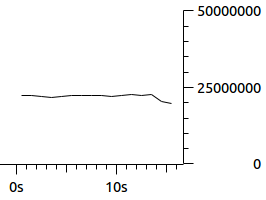
\includegraphics[width=0.25\textwidth]{images/benchmark-1/benchmark-1-s1-bs1387.png}
&
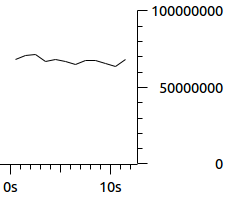
\includegraphics[width=0.2\textwidth]{images/benchmark-1/benchmark-1-s1-bs8192.png} \\ \hline
\end{tabular}
\end{table}

\begin{table}[H]
\centering
\begin{tabular}{|l|l|} \hline
16384 ($\sim$130 Msgs)& 56769 ($\sim$450 Msgs)\\ \hline
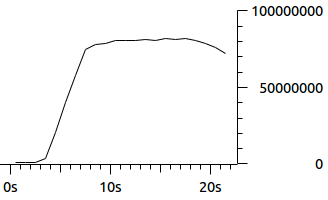
\includegraphics[width=0.25\textwidth]{images/benchmark-1/benchmark-1-s1-bs16384.png}
&
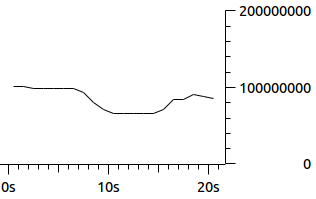
\includegraphics[width=0.25\textwidth]{images/benchmark-1/benchmark-1-s1-bs56769.png} \\ \hline
\end{tabular}
\end{table}

Scenario 2, Kafka $\rightarrow$ HMB:

\begin{table}[H]
\centering
\begin{tabular}{|l|l|l|} \hline
195 (1 Msg) & 1387 ($\sim$10 Msgs)& 8192 ($\sim$65 Msgs)\\ \hline
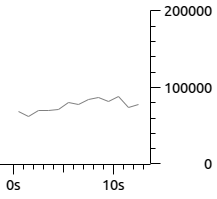
\includegraphics[width=0.2\textwidth]{images/benchmark-1/benchmark-1-s2-bs195.png}
&
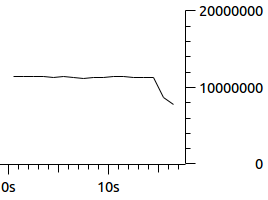
\includegraphics[width=0.25\textwidth]{images/benchmark-1/benchmark-1-s2-bs1387.png}
&
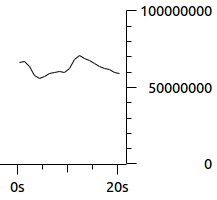
\includegraphics[width=0.2\textwidth]{images/benchmark-1/benchmark-1-s2-bs8192.png} \\ \hline
\end{tabular}
\end{table}

\begin{table}[H]
\centering
\begin{tabular}{|l|l|} \hline
16384 ($\sim$130 Msgs)& 56769 ($\sim$450 Msgs)\\ \hline
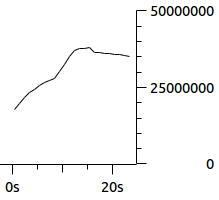
\includegraphics[width=0.2\textwidth]{images/benchmark-1/benchmark-1-s2-bs16384.png}
&
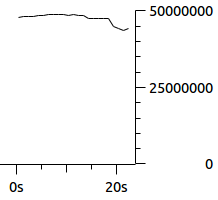
\includegraphics[width=0.2\textwidth]{images/benchmark-1/benchmark-1-s2-bs56769.png} \\ \hline
\end{tabular}
\end{table}

\newpage
Scenario 3, HMB $\rightarrow$ Kafka:

\begin{table}[H]
\centering
\begin{tabular}{|l|l|l|} \hline
195 (1 Msg) & 1387 ($\sim$10 Msgs)& 8192 ($\sim$65 Msgs)\\ \hline
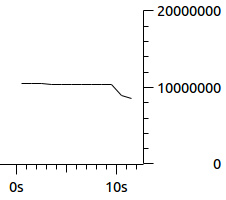
\includegraphics[width=0.2\textwidth]{images/benchmark-1/benchmark-1-s3-bs200.png}
&
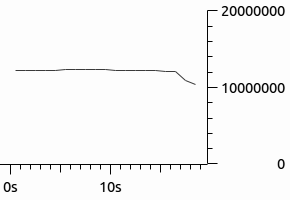
\includegraphics[width=0.25\textwidth]{images/benchmark-1/benchmark-1-s3-bs1400.png}
&
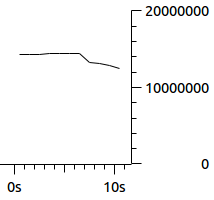
\includegraphics[width=0.2\textwidth]{images/benchmark-1/benchmark-1-s3-bs8192.png} \\ \hline
\end{tabular}
\end{table}

\begin{table}[H]
\centering
\begin{tabular}{|l|l|} \hline
16384 ($\sim$130 Msgs)& 56769 ($\sim$450 Msgs)\\ \hline
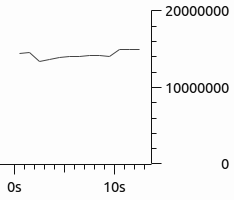
\includegraphics[width=0.2\textwidth]{images/benchmark-1/benchmark-1-s3-bs16384.png}
&
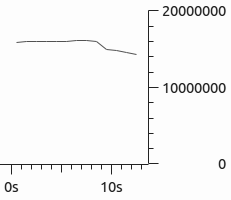
\includegraphics[width=0.2\textwidth]{images/benchmark-1/benchmark-1-s3-bs56769.png} \\ \hline
\end{tabular}
\end{table}

Scenario 4, HMB $\rightarrow$ HMB:

\begin{table}[H]
\centering
\begin{tabular}{|l|l|l|} \hline
195 (1 Msg) & 1387 ($\sim$10 Msgs)& 8192 ($\sim$65 Msgs)\\ \hline
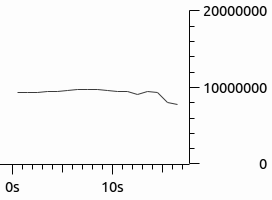
\includegraphics[width=0.2\textwidth]{images/benchmark-1/benchmark-1-s4-bs195.png}
&
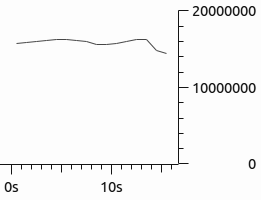
\includegraphics[width=0.25\textwidth]{images/benchmark-1/benchmark-1-s4-bs1387.png}
&
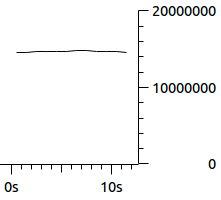
\includegraphics[width=0.2\textwidth]{images/benchmark-1/benchmark-1-s4-bs8192.png} \\ \hline
\end{tabular}
\end{table}

\begin{table}[H]
\centering
\begin{tabular}{|l|l|} \hline
16384 ($\sim$130 Msgs)& 56769 ($\sim$450 Msgs)\\ \hline
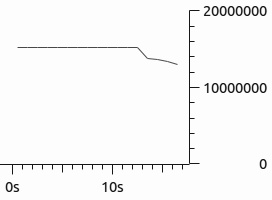
\includegraphics[width=0.2\textwidth]{images/benchmark-1/benchmark-1-s4-bs16384.png}
&
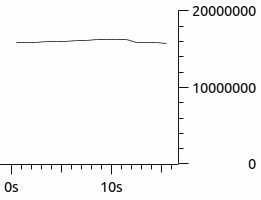
\includegraphics[width=0.2\textwidth]{images/benchmark-1/benchmark-1-s4-bs56769.png} \\ \hline
\end{tabular}
\end{table}

\newpage
\subsubsection{Conclusion}
\begin{table}[H]
\centering
\begin{tabular}{|l|l|l|l|l|}
\hline
{\bf Benchmark Variable} & \multicolumn{4}{c|}{{\bf Avg. Throughput {[}MB/s{]}}} \\ \hline \hline
Batch Size [Byte]        & Scenario 1       & Scenario 2       & Scenario 3   & Scenario 4   \\ \hline
195  (1 Msg)             & 9                & 8                & 10           & 9            \\ \hline
1387 ($\sim$10 Msgs)     & 24               & 12               & 11           & 16           \\ \hline
8192 ($\sim$65 Msgs)     & 68               & 54               & 13           & 15           \\ \hline
16384 ($\sim$130 Msgs)   & 80               & 32               & 14           & 16           \\ \hline
56769 ($\sim$450 Msgs)   & 98               & 48               & 16           & 17           \\ \hline
\end{tabular}
\end{table}
\captionof{table}{Results of benchmark "Effect of Producer Batch size"}

The result of this benchmark demonstrates the positive effect to the throughput
by increasing the producing batch size. The original Kafka setup (scenario 1),
shows a significant rise by increasing the batch size. However the
HMB setup (scenario 4) cannot use batching to full capacity. Obviously this
benchmark exposes the HMB producer as major bottleneck. Using the Kafka
producer to the HMB broker (scenario 2) gives lot better results instead of
using the HMB producer. Scenario 3 approves this suspicion. The handling
of requests on the HMB broker is quite efficient but there is still a demand
for further optimizations to get same performance than Kafka.

\subsubsection{Consequences}
During the benchmark it was conspicuous that the HMB broker is
not using full capacity of CPU. While Kafka is obviously getting use of
multi-threading, at HMB the most load weigh on a single thread. This is why
there is only one API handler thread running at the time, which is definitely
a point to optimize in future.

TODO: Figure of CPU workload

Another point with demand to optimization is the producer which manifests a
bottleneck with messages of 100 bytes (when the message size gets bigger, the
result is much better! ref). Because the provided HMB producer is quite simple
(actually just built to test), another task for the futur is to work off details for
optimized producer client which would definitely lead to better results. 

\newpage
\subsection{Producer Benchmark "Effect of Message size"}
\label{sec:conc-benchmark-2}
The goal of this benchmark is to analyze the network throughput between
producer client and broker system. The focus lies on the effect of changing the
size of a single message to the resulting transmission of bytes per
second. Persisting performance on the broker is not considered in
this benchmark.

\subsubsection{Conditions}
\begin{table}[H]
\begin{tabular}{|l| p{12cm}|} \hline
{\bf Message Size}   & 10 | 100 | 1000 | 10000 | 100000 | Bytes \\ \hline
{\bf Batch Size}     & 12800 \\ \hline
{\bf Tested Clients} &
    \begin{itemize}
        \item Kafka PerformanceProducer 2.10-0.8.2.0, single threaded
        \item HMB Producer, single threaded
    \end{itemize}\\ \hline
{\bf Tested Brokers} &
    \begin{itemize}
        \item Kafka Broker 2.10-0.8.2.0, no replication, one partition
        \item HMB Broker, no replication, one partition
    \end{itemize}\\ \hline
{\bf Measurement} & Resulting TCP throughput over a period of 10 seconds, analyzed with
    Wireshark. \\ \hline
{\bf Scenarios} & Producing as much messages as possible from client (left) to broker (right).
    The size of a messages varies in defined steps. The batch size thereby is a fixed value. 
  \begin{enumerate}
        \item Kafka Performance Producer $\rightarrow$ Kafka Broker
        \item Kafka Performance Producer $\rightarrow$ HMB Broker
        \item HMB Produer $\rightarrow$ Kafka Broker
        \item HMB Produder $\rightarrow$ HMB Broker
    \end{enumerate} \\ \hline
\end{tabular}
\end{table}
\captionof{table}{Benchmark conditions "Effect of Message size"}

\subsubsection{Results}
\begin{table}[H]
\centering
\begin{tabular}{|l|l|l|l|l|}
\hline
{\bf Benchmark Variable} & \multicolumn{4}{c|}{{\bf Avg. Throughput {[}MB/s{]}}} \\ \hline
Message Size             & Scenario 1       & Scenario 2       & Scenario 3     & Scenario 4 \\ \hline
10 B                     &                  &                  & 0              &           \\ \hline
100 B                    & 0                & 0                & 0              &            \\ \hline
1000 B (1 KB)            & 0                & 0                & 0              &            \\ \hline
10000 B (10 KB)          & 0                & 0                & 0              &            \\ \hline
100000 B (100 KB)        & 0                & 0                & 0              &             \\ \hline
1000000 (1 MB)           & 0                & 0                & 0              &             \\ \hline
\end{tabular}
\end{table}
\captionof{table}{Results of benchmark "Effect of Message size"}

%\subsection{Benchmark "Encode/Decode"}

%\subsection{Network Throughput}
%The socket based communication must not be a bottleneck in a high performance
%broker. A producer should be able to send with near the maximal throughput of
%its local network card, whereas the broker needs to handle the incoming data
%streams as fast as possible. If the limits of a single network connection is
%reached, the next step to improve performance is to balance the data
%stream on multiple replicated brokers.

%To test the network throughput for this thesis, a benchmark producer
%which identify the limits is provided.



%The variance seems to be due to Linux's I/O management facilities that batch
%data and then flush it periodically.
%-> Durchgeführte Tests 

%-> Resultat Network Throuput 

%-> Resultat Writing to the log 
%-> Vergleich Kafka (ref to Blog) 

%\begin{table}[h]
%\begin{tabular}{|c|c|c|c|}
%\hline
%{\bf Request Size (with ReqHeader)} & {\bf Message Size {[}Byte{]}} & {\bf Batch Size} & {\bf \begin{tabular}[c]{@{}c@{}}Avg. Throughput\\ {[}MB/s{]}\end{tabular}} \\ \hline
%150 B                               & 100                           & 1                & 27                                                                         \\ \hline
%1050 B                              & 100                           & 10               & 22                                                                         \\ \hline
%10.050 KB                           & 100                           & 100              & 30                                                                         \\ \hline
%100.050 KB                          & 100                           & 1000             & 32                                                                         \\ \hline
%1 MB                                & 100                           & 10000            & 40                                                                         \\ \hline
%550 B                               & 500                           & 1                & 66                                                                         \\ \hline
%1050 B                              & 500                           & 2                & 81                                                                         \\ \hline
%10.050 B                            & 500                           & 20               & 80                                                                         \\ \hline
%100.050 KB                          & 500                           & 200              & 96                                                                         \\ \hline
%1 MB                                & 500                           & 2000             & 68                                                                         \\ \hline
%1050 B                              & 1000                          & 1                & 104                                                                        \\ \hline
%10.050 B                            & 1000                          & 10               & 110                                                                        \\ \hline
%100.050 KB                          & 1000                          & 100              & 112                                                                        \\ \hline
%1 MB                                & 1000                          & 1000             & 87                                                                         \\ \hline
%10.050 B                            & 10000                         & 1                & 117                                                                        \\ \hline
%100.050 KB                          & 10000                         & 10               & *                                                                          \\ \hline
%1 MB                                & 10000                         & 100              & *                                                                          \\ \hline
%\end{tabular}
%\end{table}


\section{Outlook}

What are the next steps? As described in section \ref{sec:conc-results}, the
resulting broker implementation is not a finalized product -- it is a prototype.
It shows that it is feasible to develop an Apache Kafka like broker system
written in Haskell. An extendable and scalable implementation base and
architecture is provided. The provided benchmarks (\ref{sec:conc-benchmark-1}
and \ref{sec:conc-benchmark-2}) demonstrate good performance put also uncover
some major bottlenecks. We are certain that with further work one could build
the current version to an extraordinary broker system.

Summarized, the next tasks to do at the prototype would involve:
\begin{enumerate}
    \item Facing uncovered bottlenecks (see benchmarks)
    \item Implementation and handling of remaining API's
    \item Extending the log subsystem
    \item Work off more details for Client API
    \item Further optimizations
\end{enumerate}

After bringing the broker server to a stable and nearly feature complete
application, the next step would be to introduce broker replication. This task
probably is predestined for a further thesis whereas the goal is to analyze
distributed replication in detail and work out ZooKeeper
integration.

The Haskell community is very vital and active. We experienced that at the
\fnurl{ZuriHac 2015}{https://wiki.haskell.org/ZuriHac2015} (Google Zurich,
29.05.15) or \fnurl{HaskellerZ Meetup}{http://www.meetup.com/de/HaskellerZ/}
(ETH Zurich, 30.04.2015) we have participated during this thesis. The results
of this work will still be published open source through the \fnurl{GitHub
repositories}{https://github.com/hmb-ba}. The goal is to find contributors for
further development. For this reason we will also present this work in a
separate Meetup later in summer 2015. As for now, the highlight remains the
protocol implementation which has already been praised by the Haskell community
and found its contributors they helped uncovering minor issues.

